\section{RTAI - \rtai}
The development of \rtai (RTAI) was started just about the year 2000 by Professor Mantegazza at Dipartimento di Ingegneria Aerospaziale in Mailand. Also note that it is a fork from \rtlinux. The following architectures are supported by RTAI 5.1 are listed below\cite{rtaiHomePage}:
\begin{itemize}
    \item x86 (with and without FPU and TSC)
    \item x86\_64
    \item PowerPC
    \item ARM (StrongARM; ARM7: clps711x-family, Cirrus Logic EP7xxx, CS89712, PXA25x)
    \item m68k (supporting both MMU and NOMMU cpus)
\end{itemize}
\begin{figure}[!htbp]
    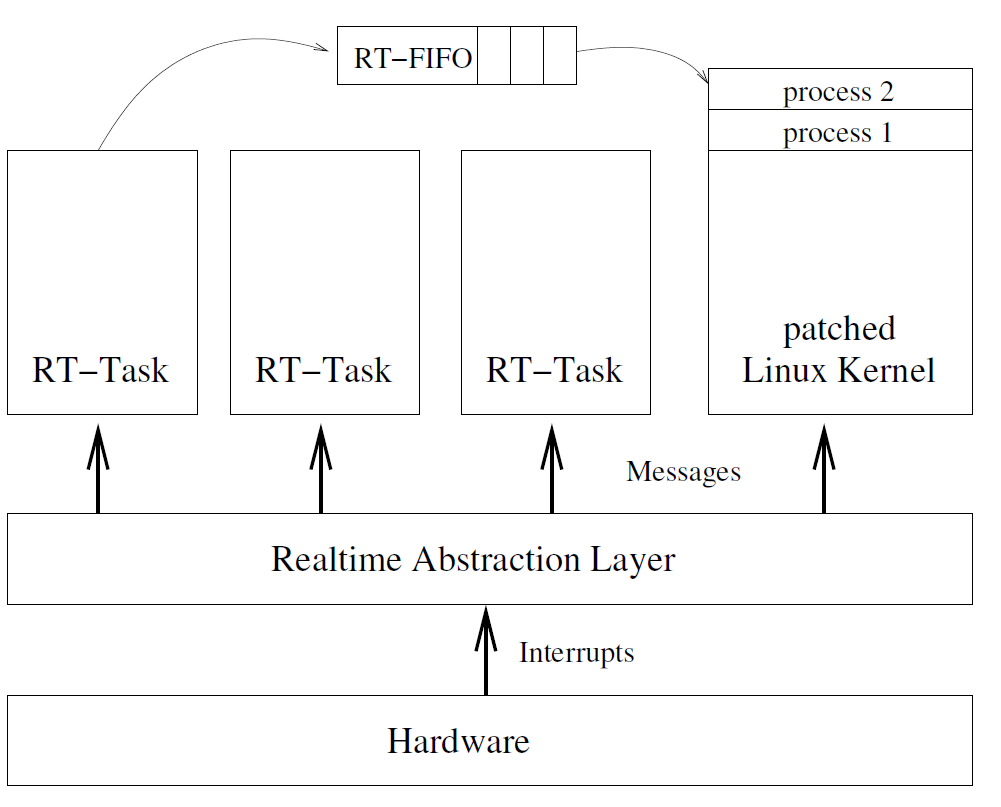
\includegraphics[width=\linewidth]{rtaiArchitecture}
    \caption{RTAI Architecture}\label{fig:rtai-architecture}
\end{figure}
Strictly speaking, it RTAI not a real time operating system, such as VXworks or QNX. It is based on the Linux kernel, providing the ability to make it fully pre-emptable.

Linux faces lack of real time support. To obtain timing correctness behavior, it is necessary to make some changes in the kernel sources, i.e. in the interrupt handling and scheduling policies. 

RTAI provides the same services as of the linux kernel core listed below:
\begin{itemize}
    \item hardware management layer dealing with event polling or processor/peripheral interrupts
    \item scheduler classes dealing with process activation, priorities, time slice
    \item communications means among applications
\end{itemize}

The kernel components of the RTAI project are under the GNU General Public License (GPL). The User-Space libraries are under the terms of the GNU Lesser General Public License (LGPL). Thus, it is possible to distribute proprietary hard realtime User-Space applications based on RTAI/LXRT and/or RTDM.

RTAI mainly traps the peripherals interrupts and if necessary re-routes them to Linux. It is not an intrusive modification of the kernel; it uses the concept of HAL (hardware abstraction layer) to get information from Linux and to trap some fundamental functions. This HAL provides few dependencies to Linux Kernel. This leads to a simple adaptation in the Linux kernel, an easy RTAI port from version to version of Linux and an easier use of other operating systems instead of RTAI. RTAI considers Linux as a background task running when no real time activity occurs.

RTAI offers a testsuite called "Showroom", which covers almost every feature available in
RTAI. It is very useful for testing the proper functionality of RTAI and can be also used for
basic measurements, e.g. scheduling latencies, under different circumstances.
\begin{figure}[!htbp]
    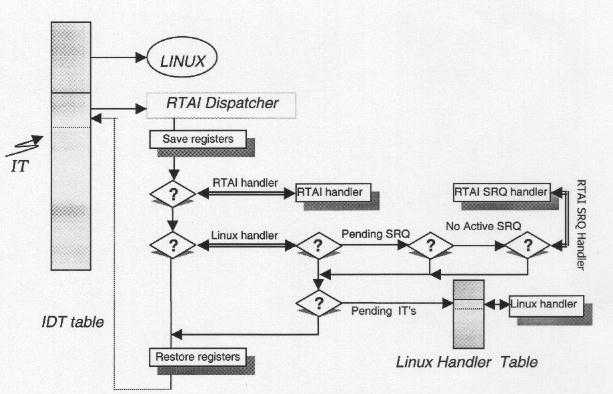
\includegraphics[width=\linewidth]{rtaiInterruptDispatcher}
    \caption{RTAI Interrupt Dispatcher\cite{rtaiPresentation}}\label{fig:rtai-interrupt-dispatcher}
\end{figure}
In order to dispatch external events in a prioritized manner, Adeos offers the possibility for stalling events. That means, during interrupt handling in stage "$ n $", domain "$ n $" can block interrupt propagation for all stages "$ k, k > n $", providing domain "$ 0 $" is the one owning the highest priority.
Interrupts are simply stored in a per-CPU log file and are dispatched after calling a special Adeos unstall routine. As a consequence of this, a standard Linux kernel blocking interrupts for performing critical sections, does not influence realtime tasks embodied in a domain lying ahead of it in the interrupt pipeline.

\subsection{Scheduling}
The scheduler is the heart of RTAI, it provides trough a series of mechanisms the real-time capabilities which are peculiar to this project. By using the RTAI scheduler the process can meet hard real time constraints and being able to run deterministically, that means that the process can be executed precisely as designed and not limited by the general purpose GNU/Linux scheduler. A real-time process which links to RTAI can therefore used to control complex applications, such as numerical control, industrial process and any complex task which requires “correct” scheduling. 

RTAI provides symmetric hard real time services inter/intra user/kernel space. Such a support comes through two schedulers, that at the moment are called $ rtai\_lxrt $ and $ rtai\_sched $. They can operate in both user and kernel mode and they differ only in relation to the objects they can schedule. That means that $ rtai\_lxrt  $is simply a GNU/Linux co-scheduler, this means that it supports hard real time for all Linux schedulable objects like processes/threads/kthreads. The $ rtai\_sched $ instead supports not only hard real time for all Linux schedulable objects, like processes/threads/kthreads, but also for RTAI own kernel tasks, which are very light kernel space only schedulable objects proper to RTAI.

Note that the big advantage of RTAI's light kernel tasks is their \textbf{fast switching time} with respect to Linux kernel threads, but on the other side it's important to know that they operate outside any Linux environment. This behavior requires some special care if one needs to inter-operate with Linux.

\section{Performance Analysis}\label{sec:performance-analysis}
In order to draw conclusions about the performance, parameters have to be defined which are important in a realtime environment. Basically, this paper deals with external interrupt latencies and scheduling latencies. Other parameters which can give information about the quality of real time capabilities are for example context switch times, process dispatch latencies or the time that is needed to allocate a certain amount of memory. 

\subsection{Parameters for performance measurement}
Before discussing the trade-off of both \rtos \space first of all it is necessary to describe the parameters and their affect on measurement of \rtos.
\begin{enumerate}
    \item Interrupt latency
        \\ In general interrupt latency is also known as interrupt response time, is the \textit{length of time that it takes for a computer interrupt to be acted on after it has been generated}. In most computers, a trade-off exists among interrupt latency, throughput, and processor utilization.
        \\ The measurement of the response time to external interrupts gives a good idea about realtime capabilities.
    \item Scheduling latency
        \\ In general, Scheduling latency refers to that \textit{time from when a task is ready to run to when it is actually gets CPU time}. 
\end{enumerate}



\section{Conclusion}
The aim of the reported work has been the  performance evaluation of Real Time Linux and RTAI(\rtai), for this evaluation we have started with basics of both \rtlinux \space and RTAI, in this basic discussion the working procedure of both the real time systems are included. Section \ref{sec:performance-analysis} includes the performance analysis focusing on mainly two performance parameters -- interrupt latency and scheduling latency.